\documentclass[conference,a4paper]{IEEEtran}

% ============================================================ Paquets
\usepackage[utf8]{inputenc}
\usepackage[T1]{fontenc}
\IfFileExists{french.ldf}{\usepackage[french]{babel}}{\usepackage[english]{babel}}
\usepackage{amsmath,amssymb}
\usepackage{graphicx}
\graphicspath{{figures/}{../figures/}}
\usepackage{booktabs,array}
\usepackage{xcolor}
\usepackage{tikz}
\usetikzlibrary{positioning,arrows.meta,calc,babel}
\usepackage{pgfplots}
\pgfplotsset{compat=1.17}
\usepackage{cite}
\usepackage{url}
% Placement des flottants : moins de blancs en bas de colonne
\renewcommand{\topfraction}{0.9}
\renewcommand{\textfraction}{0.07}
\renewcommand{\floatpagefraction}{0.85}
\setcounter{topnumber}{3}
\setcounter{totalnumber}{5}

% Couleurs du modèle : titre et intertitres en bleu
\definecolor{ieeeblue}{HTML}{1F4E79}
\definecolor{boxblue}{HTML}{DCEBF7}
\definecolor{boxgreen}{HTML}{DFF0E3}
\definecolor{boxviolet}{HTML}{E9E1F5}
\definecolor{boxorange}{HTML}{FCE8D0}
\definecolor{seriesblue}{HTML}{257DE0}
\definecolor{seriesorange}{HTML}{F47230}
\newcommand{\sect}[1]{\section{\textcolor{ieeeblue}{#1}}}
\newcommand{\subsect}[1]{\subsection{\textcolor{ieeeblue}{#1}}}
\newcommand{\code}[1]{\texttt{#1}}
\renewcommand{\figurename}{Figure}
\renewcommand{\tablename}{Tableau}

\begin{document}

\title{\textcolor{ieeeblue}{Priorisation des classes Java à risque de défaut par représentations spatio-temporelles,
fusion guidée par similarité et apprentissage contrastif : PRIORITEST-STAR}}

\author{\IEEEauthorblockN{Ayman El Garnaoui, mohamed aouijil , abdelghafoura mikali , Diae-Eddine Abou Ameur}
\IEEEauthorblockA{École Marocaine des Sciences de l'Ingénieur (EMSI) Marrakech\\
Filière Informatique et Réseaux, option Data \& IA -- 2026/2027\\
Encadrement : [à compléter]}}

\maketitle

% ------------------------------------------------------------ Résumé
\begin{abstract}
Le budget de test étant limité, une équipe doit choisir quelles classes inspecter en priorité. PRIORITEST-STAR classe
les classes Java d'une version selon leur risque de contenir un défaut, à partir de deux vues : une vue temporelle
(20 métriques orientées objet sur trois versions, encodées par un réseau convolutif temporel causal) et une vue
structurelle (le graphe des \code{import} Java, encodé par un GraphSAGE compact). L'accord cosinus entre les vues
guide leur fusion, et le modèle est entraîné avec une entropie croisée, une perte contrastive InfoNCE inter-vues et une
perte de classement RankNet. L'évaluation sur PROMISE suit un protocole chronologique strict, avec un réglage à budget
égal pour tous les modèles, 10 graines, des intervalles de confiance par bootstrap et des tests appariés. Sur Ant, aucun
mécanisme de STAR n'apporte de gain significatif : toutes les variantes font jeu égal avec une régression logistique
(précision moyenne $\approx0{,}80$). Sur Camel, la plus grande version de test, STAR avec le graphe d'imports dépasse la
régression logistique d'environ $+0{,}09$ de précision moyenne ($p\le0{,}01$), grâce à un signal de connectivité que
les métriques ne contiennent pas. Trier les classes par risque par ligne de code trouve 2,5 fois plus de défauts à
budget égal. La valeur de STAR dépend donc du projet, et le protocole permet d'expliquer quand elle apparaît.
\end{abstract}

\begin{IEEEkeywords}
prédiction de défauts logiciels, priorisation des tests, réseau convolutif temporel, GraphSAGE, apprentissage
contrastif, évaluation sensible à l'effort.
\end{IEEEkeywords}

% ------------------------------------------------------------ I. Introduction
\sect{Introduction}
Un défaut découvert tard dans le cycle de développement coûte cher, et une équipe ne peut pas tester toutes les classes
avec le même soin. La \emph{prédiction de défauts} oriente l'effort de test vers les classes les plus susceptibles d'être
défectueuses à partir de mesures du code~\cite{menzies2007}. Deux difficultés rendent le problème plus exigeant qu'une
simple classification. D'abord, il s'agit d'un \emph{classement sous budget} : les grandes classes sont plus souvent
défectueuses, mais elles coûtent aussi plus cher à inspecter~\cite{mende2010,kamei2013}. Ensuite, une classe a un
\emph{historique} (l'évolution de ses métriques d'une version à l'autre) et une \emph{position} dans l'architecture (les
classes qu'elle importe).

\begin{figure}[t]
\centering
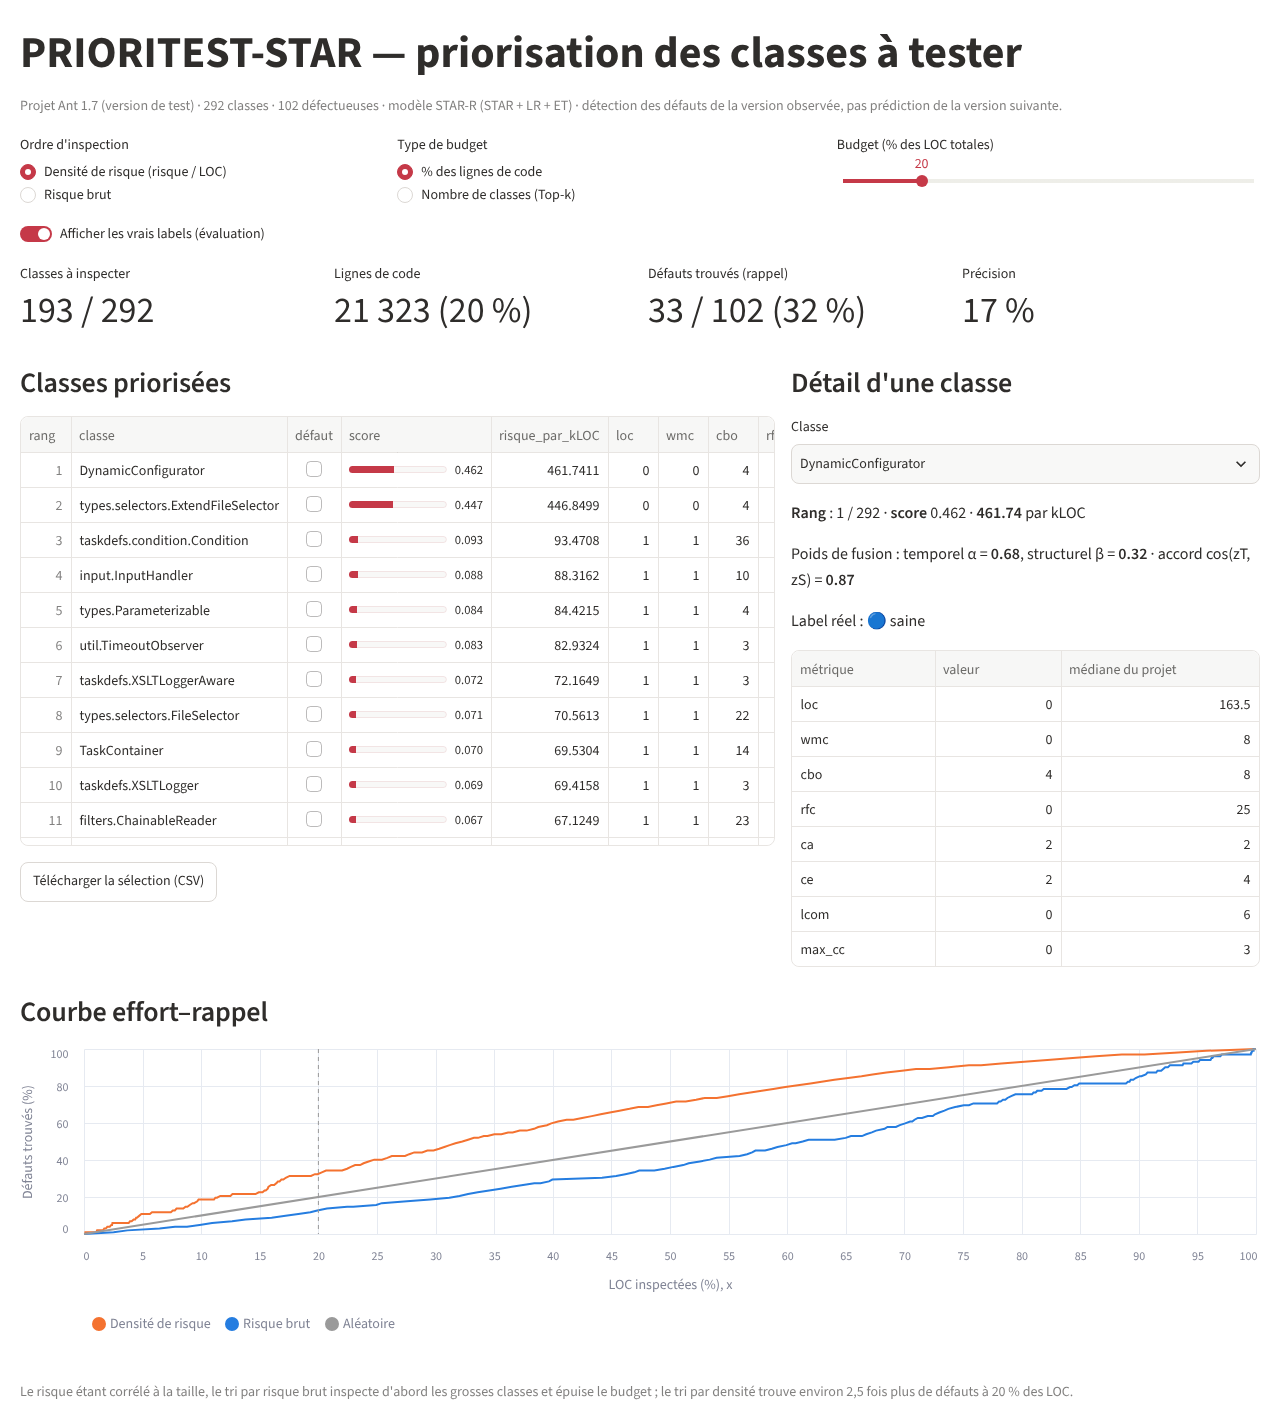
\includegraphics[width=\linewidth]{app_screenshot.png}
\caption{Application de priorisation développée : un testeur choisit un budget en lignes de code et obtient la liste des
classes à inspecter en premier, avec leur score de risque.}
\label{fig:app}
\end{figure}

\subsect{Problématique}
Une fusion guidée par la similarité entre une vue temporelle et une vue structurelle, renforcée par un alignement
contrastif inter-vues, améliore-t-elle le classement sensible à l'effort des classes défectueuses ? Cette hypothèse doit
être testée, non présupposée.

\subsect{Objectifs et contributions}
Notre travail apporte : (i) le modèle STAR à deux vues, avec fusion guidée par l'accord cosinus ; (ii) un protocole
chronologique sans fuite, où chaque modèle reçoit le même budget de réglage sur la seule validation ; (iii) une ablation
qui ajoute un mécanisme à la fois, avec intervalles de confiance et tests statistiques ; (iv) une généralisation à
quatre projets et une explication de l'apport du graphe ; (v) une application de visualisation
(figure~\ref{fig:app}).

% ------------------------------------------------------------ II. État de l'art
\sect{État de l'art}
\subsect{Métriques et classifieurs}
La suite de Chidamber et Kemerer~\cite{ck1994} et ses extensions~\cite{jureczko2010} fournissent les 20 métriques du
jeu PROMISE. Lessmann et al.~\cite{lessmann2008} observent que les écarts entre bons classifieurs sont souvent faibles,
et Tantithamthavorn et al.~\cite{tantithamthavorn2016} montrent que le réglage des hyperparamètres modifie le classement
des méthodes : une référence simple et bien réglée est indispensable.

\subsect{Similarité, graphes et effort}
Rhazi et al.~\cite{rhazi2026} apprennent la similarité \emph{entre classes} par attention inter-échantillons et vote des
plus proches voisins, avec un découpage aléatoire au sein d'une version et un F1 pondéré. Zimmermann et
Nagappan~\cite{zimmermann2008} exploitent les graphes de dépendances ; GraphSAGE~\cite{hamilton2017} en apprend des
représentations. Les TCN~\cite{bai2018} modélisent de courtes séquences, InfoNCE~\cite{oord2018} aligne des vues, et
RankNet~\cite{burges2005} apprend un ordre. Mende et Koschke~\cite{mende2010} et Kamei et al.~\cite{kamei2013}
évaluent les modèles en tenant compte de l'effort d'inspection.

\begin{table}[t]
\centering
\caption{Synthèse des travaux étudiés}
\label{tab:sota}
\footnotesize
\begin{tabular}{@{}>{\raggedright\arraybackslash}p{1.85cm}>{\raggedright\arraybackslash}p{2.55cm}>{\raggedright\arraybackslash}p{2.55cm}@{}}
\toprule
Travail & Approche & Apport pour notre étude \\
\midrule
Lessmann~\cite{lessmann2008} & 22 classifieurs & Références simples fortes \\
Rhazi~\cite{rhazi2026} & Similarité entre classes & Principe des similarités \\
Zimmermann~\cite{zimmermann2008} & Graphe de dépendances & Vue structurelle \\
Kamei~\cite{kamei2013} & Évaluation par effort & Métrique $P_{\mathrm{opt}}$ \\
\textbf{STAR} & Deux vues d'une même classe, fusion par accord & Protocole et ablation contrôlés \\
\bottomrule
\end{tabular}
\end{table}

\subsect{Positionnement}
STAR reprend le principe d'apprentissage des similarités, mais la similarité relie deux vues d'une \emph{même} classe et
sert à guider leur fusion ; ce n'est pas une reproduction de~\cite{rhazi2026}. L'évaluation est chronologique et
sensible à l'effort.

% ------------------------------------------------------------ III. Données
\sect{Données et protocole}
\subsect{Jeu PROMISE et fenêtres}
Pour une version cible $v_t$, une \emph{fenêtre stricte} réunit les classes présentes en $v_{t-2}$, $v_{t-1}$ et $v_t$ :
l'entrée temporelle est $X\in\mathbb{R}^{N\times3\times20}$, le label vaut 1 si la classe a au moins un défaut en $v_t$,
le graphe contient une arête $(i,j)$ si $i$ importe $j$, et le coût d'inspection est le nombre de lignes de code (LOC).
La normalisation est ajustée sur la seule fenêtre d'entraînement (tableau~\ref{tab:data}).

\begin{table}[t]
\centering
\caption{Fenêtres utilisées ($N$ : classes ; $P$ : défectueuses)}
\label{tab:data}
\footnotesize
\begin{tabular}{@{}llrrr@{}}
\toprule
Projet & Rôle (version) & $N$ & $P$ & \% déf. \\
\midrule
Ant   & entraînement (1.5) & 118 & 20  & 16,9 \\
Ant   & validation (1.6)   & 167 & 60  & 35,9 \\
Ant   & test (1.7)         & 292 & 102 & 34,9 \\
Camel & entraînement (1.4) & 252 & 57  & 22,6 \\
Camel & test (1.6)         & 565 & 127 & 22,5 \\
POI   & entraînement (2.5) & 224 & 153 & 68,3 \\
POI   & test (3.0)         & 311 & 202 & 65,0 \\
JEdit & test (4.3)         & 179 & 5   & 2,8 \\
\bottomrule
\end{tabular}
\end{table}

\subsect{Protocole sans fuite}
Il s'agit d'une \emph{détection} des défauts de la version observée, non d'une prédiction de la version suivante. Tous
les choix (époque, poids des pertes, seuil, mélange) sont faits sur la validation, puis le test est évalué une seule fois.
Quatre tests automatiques vérifient que les scripts de recherche n'ouvrent jamais la version de test. La
figure~\ref{fig:pipeline} résume la chaîne de traitement.

\begin{figure}[t]
\centering
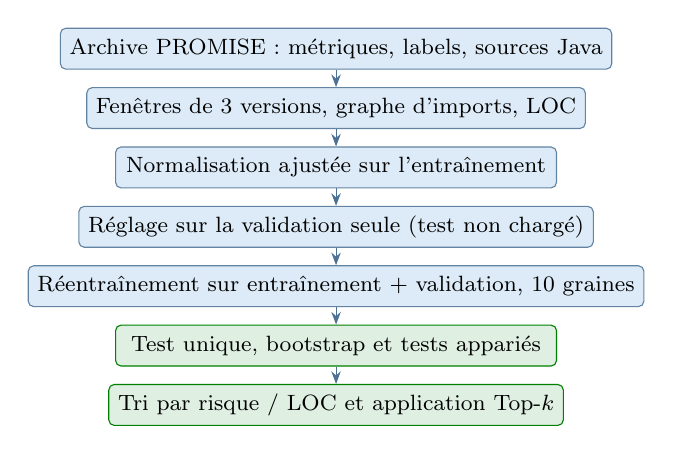
\begin{tikzpicture}[node distance=2.2mm,
  st/.style={draw=ieeeblue!70, fill=boxblue, rounded corners=2pt, minimum width=5.6cm, minimum height=5.2mm,
             font=\footnotesize, align=center},
  ar/.style={-{Stealth[length=1.6mm]}, ieeeblue!80}]
  \node[st] (a) {Archive PROMISE : métriques, labels, sources Java};
  \node[st, below=of a] (b) {Fenêtres de 3 versions, graphe d'imports, LOC};
  \node[st, below=of b] (c) {Normalisation ajustée sur l'entraînement};
  \node[st, below=of c] (d) {Réglage sur la validation seule (test non chargé)};
  \node[st, below=of d] (e) {Réentraînement sur entraînement + validation, 10 graines};
  \node[st, below=of e, fill=boxgreen, draw=green!50!black] (f) {Test unique, bootstrap et tests appariés};
  \node[st, below=of f, fill=boxgreen, draw=green!50!black] (g) {Tri par risque / LOC et application Top-$k$};
  \foreach \u/\v in {a/b,b/c,c/d,d/e,e/f,f/g} \draw[ar] (\u) -- (\v);
\end{tikzpicture}
\caption{Chaîne de traitement et protocole d'évaluation.}
\label{fig:pipeline}
\end{figure}

% ------------------------------------------------------------ IV. Architecture
\sect{Architecture proposée}
\subsect{Deux encodeurs}
La vue temporelle passe dans deux convolutions 1D causales (noyau 2, dilatations 1 et 2, 32 canaux) : la sortie à la
version $t$ ne voit que les versions $\le t$, et le dernier état donne $z_T\in\mathbb{R}^{32}$. La vue structurelle
part des métriques de $v_t$ et applique deux agrégations \emph{mean} sur le graphe d'imports pour obtenir
$z_S\in\mathbb{R}^{32}$ (figure~\ref{fig:archi}).

\begin{figure}[t]
\centering
\resizebox{\linewidth}{!}{%
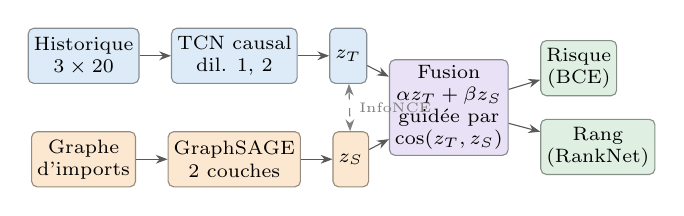
\begin{tikzpicture}[node distance=3mm and 4mm,
  bx/.style={draw=#1!60!black, fill=#1, rounded corners=2pt, align=center, font=\scriptsize,
             minimum height=7mm, inner sep=2pt},
  ar/.style={-{Stealth[length=1.5mm]}, black!65}]
  \node[bx=boxblue] (h) {Historique\\ $3\times20$};
  \node[bx=boxblue, right=of h] (tcn) {TCN causal\\ dil. 1, 2};
  \node[bx=boxblue, right=of tcn] (zt) {$z_T$};
  \node[bx=boxorange, below=6mm of h] (g) {Graphe\\ d'imports};
  \node[bx=boxorange, right=of g] (sage) {GraphSAGE\\ 2 couches};
  \node[bx=boxorange, right=of sage] (zs) {$z_S$};
  \node[bx=boxviolet, right=5mm of $(zt)!0.5!(zs)$] (fus) {Fusion\\ $\alpha z_T+\beta z_S$\\ guidée par\\ $\cos(z_T,z_S)$};
  \node[bx=boxgreen, right=of fus, yshift=5mm] (r) {Risque\\ (BCE)};
  \node[bx=boxgreen, right=of fus, yshift=-5mm] (k) {Rang\\ (RankNet)};
  \draw[ar] (h)--(tcn); \draw[ar] (tcn)--(zt); \draw[ar] (g)--(sage); \draw[ar] (sage)--(zs);
  \draw[ar] (zt)--(fus); \draw[ar] (zs)--(fus); \draw[ar] (fus)--(r); \draw[ar] (fus)--(k);
  \draw[{Stealth[length=1.5mm]}-{Stealth[length=1.5mm]}, dashed, black!50] (zt)--node[right,font=\tiny]{InfoNCE}(zs);
\end{tikzpicture}}
\caption{Architecture STAR : la flèche pointillée indique la perte contrastive inter-vues.}
\label{fig:archi}
\end{figure}

\subsect{Fusion guidée par la similarité}
L'accord entre les vues est $a_i=\cos(z_T^{(i)},z_S^{(i)})$. Un MLP produit les poids de fusion
\begin{equation}
(\alpha_i,\beta_i)=\mathrm{softmax}\big(\mathrm{MLP}([z_T^{(i)},z_S^{(i)},a_i])\big),
\end{equation}
puis la représentation fusionnée est $z_i=\alpha_i z_T^{(i)}+\beta_i z_S^{(i)}$.
Deux têtes linéaires donnent un logit de risque $r_i$ et un score de classement $s_i$. Le modèle compte
12\,644 paramètres et s'entraîne sur CPU en quelques secondes.

% ------------------------------------------------------------ V. Fondements théoriques
\sect{Fondements théoriques}
\subsect{Agrégation sur le graphe}
Pour la couche $l$, avec $\mathcal{N}(i)$ les classes importées par $i$ :
\begin{equation}
h_i^{(l+1)}=\mathrm{ReLU}\Big(W_s^{(l)}h_i^{(l)}+W_n^{(l)}\frac{1}{|\mathcal{N}(i)|}\sum_{j\in\mathcal{N}(i)}h_j^{(l)}\Big).
\end{equation}

\subsect{Fonction de perte}
L'InfoNCE symétrique de température $\tau$ prend $(z_T^{(i)},z_S^{(i)})$ comme paire positive :
\begin{equation}
\mathcal{L}_{\mathrm{NCE}}=-\frac{1}{N}\sum_{i=1}^{N}\log
\frac{\exp\big(\cos(z_T^{(i)},z_S^{(i)})/\tau\big)}{\sum_{j}\exp\big(\cos(z_T^{(i)},z_S^{(j)})/\tau\big)}.
\end{equation}
RankNet compare des paires (défectueuse $i$, saine $j$) de la même version :
\begin{equation}
\mathcal{L}_{\mathrm{Rank}}=\frac{1}{|\mathcal{P}|}\sum_{(i,j)\in\mathcal{P}}\log\big(1+e^{-(s_i-s_j)}\big).
\end{equation}
La perte totale, avec une entropie croisée pondérée par $w_+=N_-/N_+$, est
\begin{equation}
\mathcal{L}=\mathcal{L}_{\mathrm{BCE}}+\lambda_c\,\mathcal{L}_{\mathrm{NCE}}+\lambda_r\,\mathcal{L}_{\mathrm{Rank}}.
\end{equation}

\subsect{Évaluation sensible à l'effort}
Les classes sont inspectées par ordre de densité de risque $p_i/\mathrm{LOC}_i$. $P_{\mathrm{opt}}$ normalise l'aire sous
la courbe « défauts trouvés en fonction de la part de code inspectée »~\cite{kamei2013} :
\begin{equation}
P_{\mathrm{opt}}=1-\frac{\Delta_{\mathrm{opt}}-\Delta_{\mathrm{m}}}{\Delta_{\mathrm{opt}}-\Delta_{\mathrm{pire}}},
\end{equation}
où $\Delta$ désigne l'aire sous la courbe de l'ordre optimal, du modèle et du pire ordre (1 = oracle, 0,5 $\approx$
hasard). La précision moyenne (AP) mesure la détection. Les incertitudes sont estimées par bootstrap sur les
classes~\cite{efron1993}, et les comparaisons par bootstrap apparié et test de Wilcoxon~\cite{wilcoxon1945}.

% ------------------------------------------------------------ VI. Résultats
\sect{Résultats expérimentaux}
\subsect{Ablation à réglage égal sur Ant}
Chaque modèle reçoit la même grille de réglage sur Ant 1.6, puis est testé une fois sur Ant 1.7
(tableau~\ref{tab:fair}). Aucun mécanisme n'a d'effet significatif sur l'AP ; RankNet dégrade légèrement les
résultats (A5$\to$A6 : $-0{,}008$, $p=0{,}049$). L'intervalle de confiance d'environ $\pm0{,}07$ ne permet pas de
détecter un effet inférieur à 0,03. En classement sensible à l'effort, Random Forest ($+0{,}036$, $p=0{,}007$) et le
mélange STAR + LR + ET ($+0{,}008$, $p=0{,}006$) dépassent la régression logistique.

\begin{table}[t]
\centering
\caption{Ant 1.7, réglage égal, 10 graines}
\label{tab:fair}
\footnotesize
\begin{tabular}{@{}lccc@{}}
\toprule
Modèle & AP & IC 95\,\% & $P_{\mathrm{opt}}$ \\
\midrule
A2 TCN + BCE            & 0,801 & [0,725 ; 0,865] & 0,708 \\
A3 + graphe             & 0,799 & [0,728 ; 0,866] & 0,711 \\
A4 + fusion cosinus     & 0,801 & [0,734 ; 0,866] & 0,713 \\
A5 + InfoNCE            & 0,802 & [0,734 ; 0,866] & 0,717 \\
A6 + RankNet (STAR)     & 0,794 & [0,717 ; 0,866] & 0,711 \\
Régression logistique   & 0,798 & [0,721 ; 0,865] & 0,714 \\
Random Forest           & \textbf{0,809} & [0,725 ; 0,880] & \textbf{0,750} \\
Mélange STAR + LR + ET  & 0,806 & [0,724 ; 0,874] & 0,721 \\
\bottomrule
\end{tabular}
\end{table}

\subsect{Effort d'inspection}
Trié par risque brut, le modèle fait moins bien que le hasard à budget fixé, car les classes défectueuses sont beaucoup
plus grandes (médiane de 517 LOC contre 104). Trier par densité de risque trouve 2,5 fois plus de défauts à 20\,\% du
code (0,33 contre 0,13, figure~\ref{fig:budget}). Intégrer l'effort directement dans la perte n'apporte rien de plus :
le poids appris sur $\log\mathrm{LOC}$ converge vers 1, soit la même règle.

\begin{figure}[t]
\centering
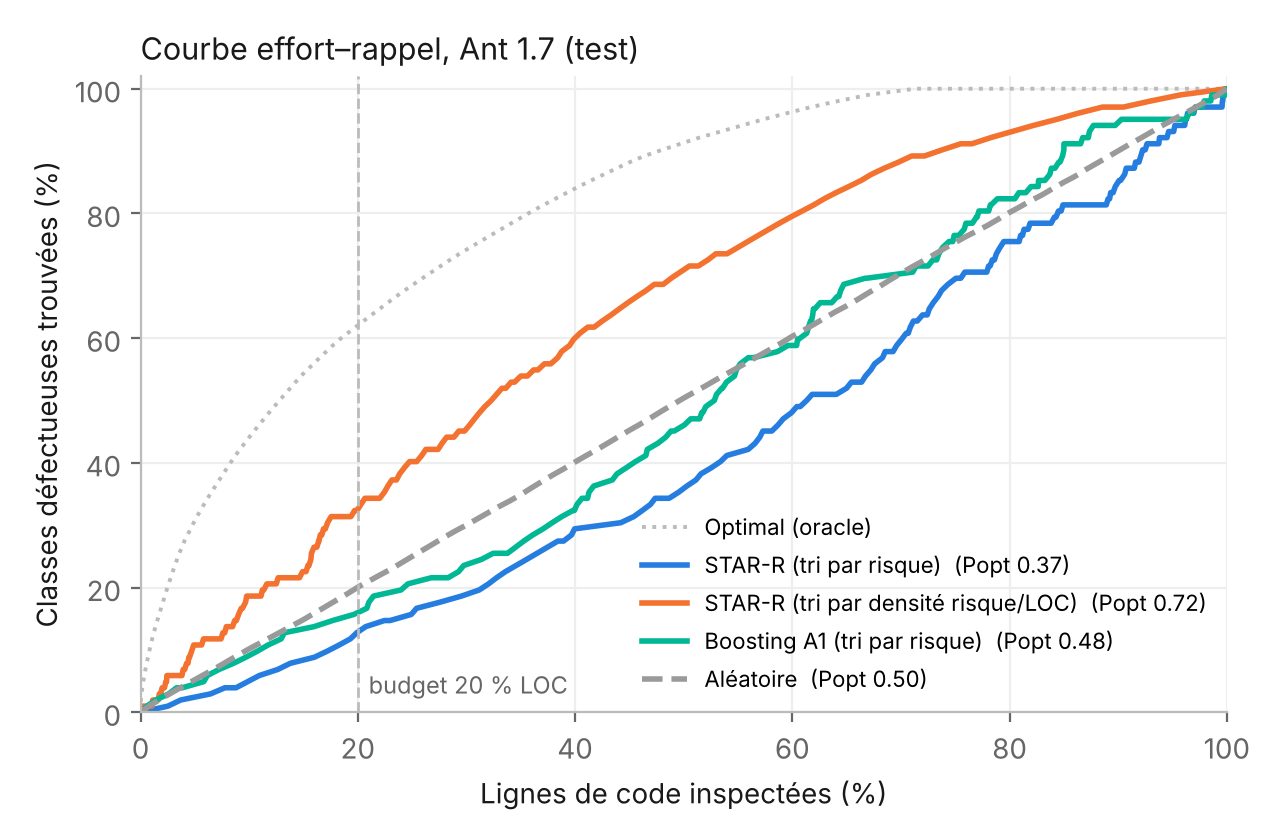
\includegraphics[width=\linewidth]{budget_recall.png}
\caption{Défauts trouvés en fonction de la part de code inspectée (Ant 1.7) : tri par densité de risque contre tri par
risque brut.}
\label{fig:budget}
\end{figure}

\subsect{Généralisation à Camel, POI et JEdit}
Réglé à l'intérieur de sa version d'entraînement, STAR dépasse nettement la régression logistique sur Camel
(tableau~\ref{tab:camel}), alors que RankNet dégrade de nouveau ($-0{,}041$, $p=0{,}011$). Sur POI, avec les réglages
d'Ant, les variantes avec graphe s'effondrent, mais STAR entraîné avec les autres projets y est le meilleur modèle
(AP 0,920) ; il exploite mieux qu'une régression logistique les données d'autres projets (Ant, POI). JEdit 4.3, avec
5 défauts, n'est pas interprétable.

\begin{table}[t]
\centering
\caption{Camel 1.6, réglage interne à Camel 1.4, écart contre LR}
\label{tab:camel}
\footnotesize
\begin{tabular}{@{}lccc@{}}
\toprule
Modèle & AP & $\Delta$AP vs LR & $p$ \\
\midrule
Régression logistique  & 0,452 & --- & --- \\
ExtraTrees             & 0,486 & $+0{,}035$ & 0,16 \\
A3 + graphe            & 0,498 & $+0{,}086$ & 0,009 \\
A5 + InfoNCE           & \textbf{0,507} & $\mathbf{+0{,}088}$ & \textbf{0,003} \\
A6 + RankNet           & 0,462 & $+0{,}047$ & 0,14 \\
Mélange STAR + LR + ET & 0,517 & $+0{,}065$ & 0,002 \\
\bottomrule
\end{tabular}
\end{table}

\subsect{Pourquoi le graphe aide sur Camel}
Sur Camel, une classe isolée dans le graphe d'imports n'est presque jamais défectueuse (1,3\,\% contre 26\,\% pour une
classe connectée), et tout le gain du graphe porte sur les classes connectées ($+0{,}052$ d'AP). Sur Ant, ce contraste
est faible et le graphe n'ajoute rien (figure~\ref{fig:graph}). Les classes défectueuses ne s'importent pas davantage
entre elles : le signal est la connectivité elle-même, que les métriques de couplage ne reflètent qu'en partie.

\begin{figure}[t]
\centering
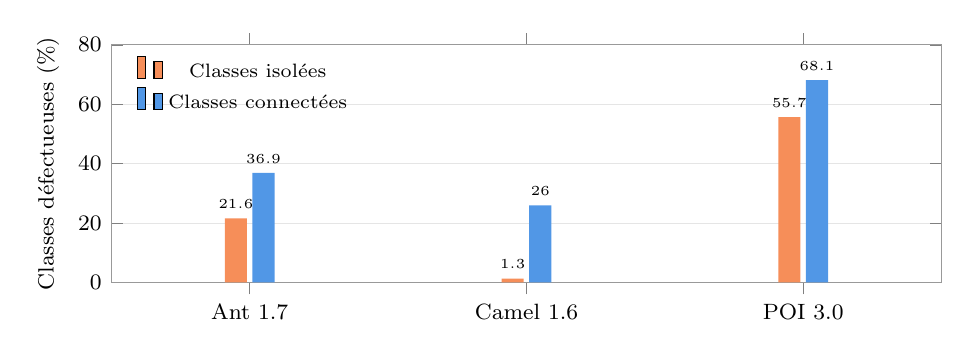
\begin{tikzpicture}
\begin{axis}[
  ybar, bar width=8pt, width=\linewidth, height=4.6cm,
  ymin=0, ymax=80, ylabel={\footnotesize Classes défectueuses (\%)},
  symbolic x coords={Ant 1.7, Camel 1.6, POI 3.0}, xtick=data,
  tick label style={font=\footnotesize}, enlarge x limits=0.25,
  legend style={font=\scriptsize, at={(0.02,0.98)}, anchor=north west, draw=none, fill=none},
  nodes near coords, nodes near coords style={font=\tiny},
  ymajorgrids, grid style={black!10}, axis line style={black!40}]
\addplot[fill=seriesorange!80, draw=none] coordinates {(Ant 1.7,21.6) (Camel 1.6,1.3) (POI 3.0,55.7)};
\addplot[fill=seriesblue!80, draw=none] coordinates {(Ant 1.7,36.9) (Camel 1.6,26.0) (POI 3.0,68.1)};
\legend{Classes isolées, Classes connectées}
\end{axis}
\end{tikzpicture}
\caption{Taux de défauts des classes isolées et connectées dans le graphe d'imports : le contraste est maximal sur
Camel, là où le graphe apporte un gain.}
\label{fig:graph}
\end{figure}

\subsect{Amélioration de la fusion}
Masquer les faux négatifs de l'InfoNCE ou ajouter un contraste supervisé ne change rien. Une régularisation par
l'entropie de la porte fait utiliser les deux vues de façon équilibrée (poids temporel de 0,63 à 0,55) sans perte de
performance ; elle est retenue pour l'interprétabilité.

% ------------------------------------------------------------ VII. Réalisations
\sect{Réalisations logicielles}
Le dépôt contient le modèle et les pertes (\code{src/model.py}), les métriques et les tests statistiques
(\code{src/stats.py}), un script par étude (comparaison équitable, effort, données inter-projets, transfert, réglage
par projet, analyse du graphe), 36 tests unitaires dont quatre tests anti-fuite, et une application Streamlit
(figure~\ref{fig:app}) qui affiche le Top-$k$ sous un budget en lignes de code. Chaque étude se relance en une commande
et en quelques minutes sur CPU.

\begin{table}[t]
\centering
\caption{Configuration retenue (choisie sur la validation)}
\label{tab:config}
\footnotesize
\begin{tabular}{@{}lc@{}}
\toprule
Paramètre & Valeur \\
\midrule
Dimension des représentations & 32 \\
Taux d'apprentissage / weight decay & $10^{-3}$ / $10^{-3}$ \\
$\lambda_c$ / $\tau$ & 0,1 / 0,2 \\
Époques (courbe moyennée et lissée) & 64 \\
Graines & 10 \\
Entraînement / validation / test (Ant) & 1.5 / 1.6 / 1.7 \\
\bottomrule
\end{tabular}
\end{table}

% ------------------------------------------------------------ VIII. Discussion
\sect{Discussion et limites}
Le protocole est volontairement strict, ce qui révèle ses propres limites. Ant ne compte que 118 classes
d'entraînement, et une seule version de test par projet donne des intervalles de confiance larges. Les classes nouvelles
sont exclues des fenêtres, d'où un biais de sélection, et le graphe d'imports est partiel. Il s'agit d'une détection sur
la version observée, pas d'une prévision. Enfin, l'explication de l'apport du graphe repose sur trois projets
informatifs : elle est corrélationnelle.

% ------------------------------------------------------------ IX. Conclusion
\sect{Conclusion}
STAR combine l'historique des métriques et la structure des imports dans un modèle compact. Avec un protocole équitable,
la réponse à la question de recherche est nuancée : sur Ant, aucun mécanisme n'apporte de gain mesurable ; sur Camel,
la vue structurelle dépasse nettement les références grâce au signal de connectivité ; et le tri par densité de risque
reste le levier le plus fort pour l'effort d'inspection. Les références à base d'arbres restent des concurrents à
toujours inclure.

% ------------------------------------------------------------ X. Travaux futurs
\sect{Travaux futurs}
\subsect{Réglage par projet}
Terminer le réglage interne sur POI pour vérifier si l'effondrement observé vient des réglages d'Ant, puis classer tous
les modèles par la méthode de Scott-Knott.

\subsect{Données et domaine}
Tirer parti des données d'autres projets par adaptation de domaine, et étudier les classes nouvelles à partir de
l'archive PROMISE complète.

\subsect{Métriques de processus}
Ajouter des métriques de changement (modifications, auteurs)~\cite{moser2008} pour mieux détecter les petites classes
défectueuses, que les métriques structurelles ne distinguent pas.

% ------------------------------------------------------------ Références
\begin{thebibliography}{99}
\bibitem{menzies2007} T.~Menzies, J.~Greenwald, and A.~Frank, ``Data mining static code attributes to learn defect
  predictors,'' \emph{IEEE Trans. Softw. Eng.}, vol.~33, no.~1, pp.~2--13, 2007.
\bibitem{mende2010} T.~Mende and R.~Koschke, ``Effort-aware defect prediction models,'' in \emph{Proc. CSMR}, 2010.
\bibitem{kamei2013} Y.~Kamei \emph{et al.}, ``A large-scale empirical study of just-in-time quality assurance,''
  \emph{IEEE Trans. Softw. Eng.}, vol.~39, no.~6, pp.~757--773, 2013.
\bibitem{ck1994} S.~R. Chidamber and C.~F. Kemerer, ``A metrics suite for object oriented design,''
  \emph{IEEE Trans. Softw. Eng.}, vol.~20, no.~6, pp.~476--493, 1994.
\bibitem{jureczko2010} M.~Jureczko and L.~Madeyski, ``Towards identifying software project clusters with regard to
  defect prediction,'' in \emph{Proc. PROMISE}, 2010.
\bibitem{lessmann2008} S.~Lessmann, B.~Baesens, C.~Mues, and S.~Pietsch, ``Benchmarking classification models for
  software defect prediction: A proposed framework and novel findings,'' \emph{IEEE Trans. Softw. Eng.}, vol.~34,
  no.~4, pp.~485--496, 2008.
\bibitem{tantithamthavorn2016} C.~Tantithamthavorn, S.~McIntosh, A.~E. Hassan, and K.~Matsumoto, ``Automated parameter
  optimization of classification techniques for defect prediction models,'' in \emph{Proc. ICSE}, 2016.
\bibitem{rhazi2026} A.-R. Rhazi, O.~Banouar, F.~Toure, and S.~Raghay, ``Software defect prediction via contrastive
  similarity learning and inter-sample attention,'' \emph{Sci. Comput. Program.}, vol.~254, p.~103534, 2026.
\bibitem{zimmermann2008} T.~Zimmermann and N.~Nagappan, ``Predicting defects using network analysis on dependency
  graphs,'' in \emph{Proc. ICSE}, 2008.
\bibitem{hamilton2017} W.~L. Hamilton, R.~Ying, and J.~Leskovec, ``Inductive representation learning on large
  graphs,'' in \emph{Proc. NeurIPS}, 2017.
\bibitem{bai2018} S.~Bai, J.~Z. Kolter, and V.~Koltun, ``An empirical evaluation of generic convolutional and
  recurrent networks for sequence modeling,'' arXiv:1803.01271, 2018.
\bibitem{oord2018} A.~van den Oord, Y.~Li, and O.~Vinyals, ``Representation learning with contrastive predictive
  coding,'' arXiv:1807.03748, 2018.
\bibitem{burges2005} C.~Burges \emph{et al.}, ``Learning to rank using gradient descent,'' in \emph{Proc. ICML}, 2005.
\bibitem{efron1993} B.~Efron and R.~J. Tibshirani, \emph{An Introduction to the Bootstrap}. Chapman \& Hall, 1993.
\bibitem{wilcoxon1945} F.~Wilcoxon, ``Individual comparisons by ranking methods,'' \emph{Biometrics Bulletin},
  vol.~1, no.~6, pp.~80--83, 1945.
\bibitem{moser2008} R.~Moser, W.~Pedrycz, and G.~Succi, ``A comparative analysis of the efficiency of change metrics
  and static code attributes for defect prediction,'' in \emph{Proc. ICSE}, 2008.
\end{thebibliography}

\end{document}
